\documentclass[a4paper,11pt]{article}

\usepackage{../../préambule}
\usepackage{colortbl}

\addtolength{\oddsidemargin}{-0.5cm}
\addtolength{\evensidemargin}{-0.5cm}
\addtolength{\textwidth}{1cm}

\makeatletter
\renewcommand{\maketitle}{%
{\scriptsize colle dans ton cahier d'exercices, et écrit dans ton cahier} \vspace{0.5em}

	\begin{center}
		\LARGE
		\myuline{\@title}
		\vspace{2em}
	\end{center}
}
\makeatother

\usetikzlibrary{shadows,shapes,positioning}

\tikzstyle{shadowtext} = [
	draw=black,
	fill=white,
	rectangle,
	inner sep=10pt,
	style=rounded corners,
	drop shadow={fill=gray,opacity=0.8}
]

\title{Activité : situations de proportionnalité}
\date{}
\author{}

\begin{document}

\maketitle

\begin{exercice}
	Alan aime beaucoup le vélo. Dès sa première semaine de vacances, il en a fait pendant 3 jours de suite :

	\begin{tabular}{|c|c|c|c|}
		\hline
		                                           & \cellcolor{lightgray} Lundi & \cellcolor{lightgray} Mardi & \cellcolor{lightgray} Mercredi \\ \hline
		\cellcolor{lightgray} Temps (en heures)    & 2                           & 3                           & 5                              \\ \hline
		\cellcolor{lightgray} kilomètres parcourus & 46                          & 69                          & 115                            \\ \hline
	\end{tabular}
	\begin{enumerate}
		\item Pour chaque jour du tableau, calculer la grandeur \textbf{distance ÷ temps}.
		\item Les grandeurs de ce tableau sont-elles proportionnelles ?
	\end{enumerate}
\end{exercice}

\vspace{1.5em}

\begin{exercice}
	Regarde les figures suivantes : \vspace{1em}

	\begin{center}
		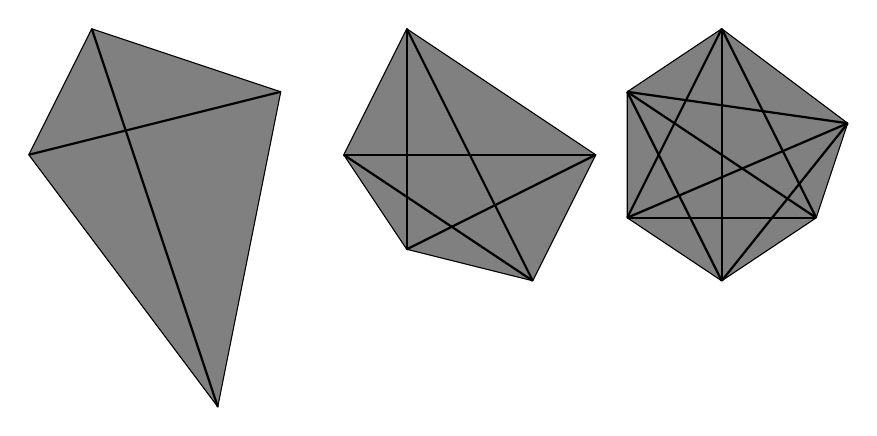
\begin{tikzpicture}[scale=0.8]
			\coordinate (tetra-1) at (0,0);
			\coordinate (tetra-2) at (1,2);
			\coordinate (tetra-3) at (4,1);
			\coordinate (tetra-4) at (3,-4);

			\coordinate (penta-1) at (5,0);
			\coordinate (penta-2) at (6,2);
			\coordinate (penta-3) at (9,0);
			\coordinate (penta-4) at (8,-2);
			\coordinate (penta-5) at (6,-1.5);

			\coordinate (hexa-1) at (9.5,1);
			\coordinate (hexa-2) at (11,2);
			\coordinate (hexa-3) at (13,0.5);
			\coordinate (hexa-4) at (12.5,-1);
			\coordinate (hexa-5) at (11,-2);
			\coordinate (hexa-6) at (9.5,-1);

			\draw[fill,color=gray,draw=black] (tetra-1) -- (tetra-2) -- (tetra-3) -- (tetra-4) -- cycle;
			\draw[thick,black] (tetra-1) -- (tetra-3);
			\draw[thick,black] (tetra-2) -- (tetra-4);

			\draw[fill,color=gray,draw=black] (penta-1) -- (penta-2) -- (penta-3) -- (penta-4) -- (penta-5) -- cycle;
			\draw[thick,black] (penta-1) -- (penta-3);
			\draw[thick,black] (penta-3) -- (penta-5);
			\draw[thick,black] (penta-5) -- (penta-2);
			\draw[thick,black] (penta-2) -- (penta-4);
			\draw[thick,black] (penta-4) -- (penta-1);


			\draw[fill,color=gray,draw=black] (hexa-1) -- (hexa-2) -- (hexa-3) -- (hexa-4) -- (hexa-5) -- (hexa-6) -- cycle;
			\draw[thick,black] (hexa-1) -- (hexa-3);
			\draw[thick,black] (hexa-3) -- (hexa-5);
			\draw[thick,black] (hexa-5) -- (hexa-1);
			\draw[thick,black] (hexa-2) -- (hexa-4);
			\draw[thick,black] (hexa-4) -- (hexa-6);
			\draw[thick,black] (hexa-6) -- (hexa-2);
			\draw[thick,black] (hexa-1) -- (hexa-4);
			\draw[thick,black] (hexa-2) -- (hexa-5);
			\draw[thick,black] (hexa-3) -- (hexa-6);
		\end{tikzpicture}
	\end{center}

	\begin{enumerate}
		\item Recopie le tableau suivant dans ton cahier d'exercices, puis complète-le :

		      \begin{tabular}{|c|c|c|c|}
			      \hline
			                                                 & \cellcolor{lightgray} Quadrilatère & \cellcolor{lightgray} Pentagone & \cellcolor{lightgray}  Hexagone \\ \hline
			      \cellcolor{lightgray} Nombre de côtés      &                                    &                                 &                                 \\ \hline
			      \cellcolor{lightgray} Nombre de diagonales &                                    &                                 &                                 \\ \hline
		      \end{tabular}
		\item Y-a-t'il proportionnalité entre le nombre de côtés et le nombre de diagonales ?
	\end{enumerate}
\end{exercice}

\vspace{1.5em}

\begin{exercice}
	À divers âges de sa vie, Rémi a mesuré sa taille.

	\begin{enumerate}
		\item Avant de faire des calculs, essayons de réfléchir intuitivement : penses-tu que la taille de Rémi soit proportionnelle à son âge ?
		\item Vérifie ton hypothèse grâce au tableau suivant :

		      \begin{tabular}{|c|c|c|c|c|c|}
			      \hline
			      \cellcolor{lightgray} Âge (en années)         & 2  & 5   & 10  & 12  & 14  \\ \hline
			      \cellcolor{lightgray} Taille (en centimètres) & 80 & 100 & 125 & 150 & 165 \\ \hline
		      \end{tabular}
	\end{enumerate}

	\begin{vocabulaire}[Hypothèse]
		Quand on fait une \textbf{hypothèse}, cela veut dire qu'on pense que quelque chose est vrai, mais qu'on ne l'a pas encore prouvé.
	\end{vocabulaire}
\end{exercice}

\end{document}